\documentclass[11pt]{article}
\usepackage[a4paper,margin=22mm,headheight=16pt]{geometry}
\usepackage{fontspec,xeCJK,xcolor,graphicx,enumitem,fancyhdr,titlesec}
\usepackage{hyperref}
\IfFontExistsTF{Times New Roman}{\setmainfont{Times New Roman}}{\setmainfont{TeX Gyre Termes}}
\IfFontExistsTF{FangSong}{\setCJKmainfont[AutoFakeBold=2]{FangSong}}{\IfFontExistsTF{仿宋}{\setCJKmainfont[AutoFakeBold=2]{仿宋}}{\IfFontExistsTF{FandolFang-Regular.otf}{\setCJKmainfont[AutoFakeBold=2]{FandolFang-Regular.otf}}{\setCJKmainfont{FandolSong-Regular.otf}}}}
\definecolor{ink}{HTML}{173747}\definecolor{accent}{HTML}{227E82}
\hypersetup{colorlinks=true,urlcolor=accent,linkcolor=accent}
\linespread{1.22}\setlength{\parindent}{0pt}\setlength{\parskip}{6pt}
\setlist[itemize]{leftmargin=1.4em,itemsep=3pt}
\titleformat{\section}{\large\bfseries\color{ink}}{}{0pt}{}
\titlespacing*{\section}{0pt}{14pt}{7pt}
\pagestyle{fancy}\fancyhf{}\lhead{\small LEARNPATH / 学习手册}\rhead{\small Source-grounded learning}\cfoot{\small\thepage}
\emergencystretch=2em\widowpenalty=10000\clubpenalty=10000
\newcommand{\Needspace}[1]{\par\begingroup\dimen0=#1\relax\vskip0pt plus\dimen0\penalty-100\vskip0pt plus-\dimen0\vskip\dimen0\penalty9999\vskip-\dimen0\vskip0pt\endgroup}
\begin{document}


{\LARGE\bfseries\color{ink} 边际思维与沉没成本}\par

2026-10-08 | Day03/30 | 阅读 8 分钟 + 练习 3 分钟\par\vspace{6pt}

\Needspace{5\baselineskip}\section*{今日导航}

今天回答：已经花了很多钱，是不是就应该继续？目标是区分总量、边际量和不可收回的既往成本。先回忆昨天的面包店：决定今天多烤一盘时，老板真正面对的选择是什么？

\Needspace{5\baselineskip}\section*{把决策写成“再多一点”}

边际分析比较行动改变一单位或一小步带来的新增收益与新增成本，而不是只比较过去的总量。[S2] 图 C 的整只面包与额外一片，帮助区分这两种问题。实际的“一步”可以是一盘面包、一小时营业或一周项目试验，应与可执行选择一致。

\begin{center}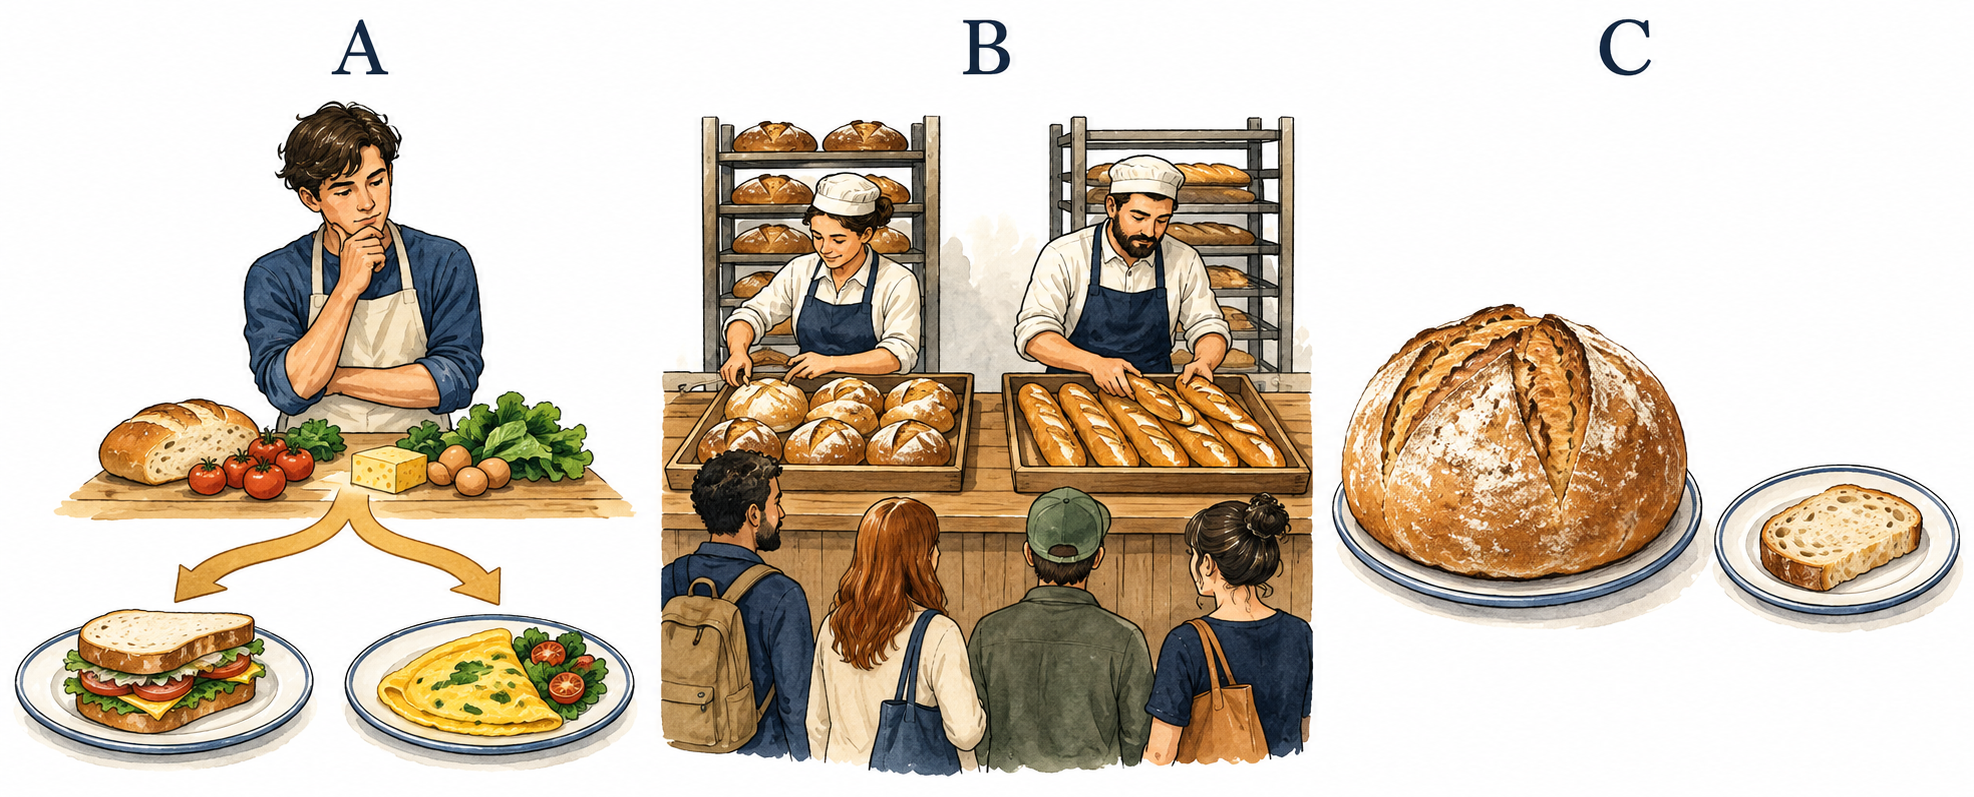
\includegraphics[width=\linewidth,height=0.26\textheight,keepaspectratio]{../assets/figure-a92b6089a95f.png}\par

{\small 本课重点看 C 区。A 同一组资源对应不同选择；B 买方与卖方共同形成市场；C 整体收益与额外一单位收益要分开计算。}\par

{\footnotesize AI生成教学示意，非实物照片、原始史料或官方架构。生成方式：内置文生图；提示词见仓库 docs/image-prompts.json。}\end{center}

\Needspace{5\baselineskip}\section*{三个判断层次}

第一，总体是否值得：开店的总体收入能否覆盖相应成本？第二，当前是否多做一步：新增这一盘会增加多少收入和成本？第三，未来是否继续：从现在起各方案的预期收益和可避免成本是什么？把这三个层次混在一起，就容易因过去投入很大而忽略未来选择。

沉没成本是已经发生且无法收回的支出。它不能因你接下来继续或停止而改变，因而不该单独成为继续的理由。但“过去买的设备”未必全部沉没：如果设备还能卖出或转用，就有当前的替代价值。情绪上的不甘与经济上的可回收价值也应分别记录。

\Needspace{5\baselineskip}\section*{教学案例：是否延长营业}

假设面包店晚关门一小时，预计新增销售收入200元，新增原料与人工合计150元，且没有其他影响。在这个简化设定中，额外收益超过额外成本50元；租金若无论是否延时都不变，就不属于这一步的新增成本。数字为教学假设。

进一步检查：延时会不会只是把原本白天的购买搬到晚上？会不会让员工第二天效率下降？食品浪费是否增加？若有这些影响，应纳入相关未来后果。边际分析要求补全决策相关项，不是看到正数就机械执行；预测不确定时，可以先短期试验再更新判断。

\Needspace{5\baselineskip}\section*{三分钟练习与自查}

你已买了一张不能退的电影票，但临时出现一个更重要的安排。请写下两个方案各自还会带来的收益和新增成本，最后指出票价为何不决定下一步。

参考：票价在两个方案下都无法收回，所以不是两者之间的差额；但交通费、时间和实际享受仍不同。如果电影票可以转让，转让收入就进入比较。自查时确认你没有把“沉没成本不决定行动”误解成“不要反思过去”：事后复盘可改善下次购买，但不能改变已发生事实。

\Needspace{5\baselineskip}\section*{复盘与明日连接}

问“从现在起会改变什么”，能把决策从过去的投入转回未来的选择。机会成本帮助识别替代方案，边际分析帮助比较下一步。明天学习弹性：价格变化相同，不同商品的购买反应为什么会相差很大？

\Needspace{6\baselineskip}\section*{扩展学习 / Further reading}\small 以下为选读，不计入每日必做时间。\begin{enumerate}[leftmargin=1.6em]

\item [S1] \href{https://openstax.org/books/principles-economics-3e/pages/1-1-what-is-economics-and-why-is-it-important}{What Is Economics, and Why Is It Important?} — 从稀缺与分工建立课程起点；文中旧统计不作为现状。\par OpenStax | 发布：未标注 | 核验：2026-10-08

\item [S2] \href{https://openstax.org/books/principles-economics-3e/pages/2-1-how-individuals-make-choices-based-on-their-budget-constraint}{Budget Constraint and Individual Choices} — 重点读机会成本、预算约束与边际分析。\par OpenStax | 发布：未标注 | 核验：2026-10-08

\item [S3] \href{https://openstax.org/books/principles-economics-3e/pages/2-2-the-production-possibilities-frontier-and-social-choices}{Production Possibilities Frontier} — 把个人选择扩展为社会资源配置，观察模型假设。\par OpenStax | 发布：未标注 | 核验：2026-10-08

\item [S4] \href{https://openstax.org/books/principles-economics-3e/pages/3-1-demand-supply-and-equilibrium-in-markets-for-goods-and-services}{Demand, Supply, and Equilibrium} — 对照需求、供给和均衡的图形定义。\par OpenStax | 发布：未标注 | 核验：2026-10-08

\item [S5] \href{https://openstax.org/books/principles-economics-3e/pages/3-2-shifts-in-demand-and-supply-for-goods-and-services}{Shifts in Demand and Supply} — 区分价格变化引起的沿曲线移动与其他条件变化引起的曲线移动。\par OpenStax | 发布：未标注 | 核验：2026-10-08

\end{enumerate}

\end{document}